\documentclass{article}
% Useful packages
\usepackage{amsmath} % Required for advanced math typesetting
\usepackage{graphicx} % Required for inserting images
\usepackage{xcolor} % Required for color definitions
\usepackage{listings}
\usepackage{tcolorbox} % Required for creating boxes
\usepackage{float} % Required for controlling the position of images


% Code settings
\lstset{
    language=C,
    basicstyle=\ttfamily\small,
    keywordstyle=\color{blue},
    commentstyle=\color{green!50!black},
    stringstyle=\color{orange},
    showstringspaces=false,
    breaklines=true,
    frame=single,
    numbers=left,
    numberstyle=\tiny,
    stepnumber=1
}

\setlength{\parindent}{0pt}

\title{SEAI\_2024\_R12}
\author{Giulio Capecchi, Jacopo Niccolai}
\date{December 2024}

\begin{document}

\maketitle


\section{Introduction}
This project focuses on the synthesis of the forward pass for three types of neural network architectures: a \textbf{Multilayer Perceptron (MLP)}, a \textbf{Convolutional Neural Network (ConvNet)}, and a \textbf{Transformer}, implemented on an FPGA.  
To achieve this, the network parameters were first obtained using Python and the \textit{PyTorch} library. These parameters were subsequently hardcoded into \texttt{C} code, enabling the hardware synthesis process.

\section{Project Description}
\subsection{Workflow Overview}
The neural networks were constructed and trained using the \textit{PyTorch} library. Once trained, the weights and biases were exported to be hardcoded into the corresponding \texttt{C} implementation. The \texttt{C} code was specifically designed to be compatible with FPGA synthesis tools, such as Vitis HLS, ensuring efficient hardware synthesis.


\subsection{C Implementation}
The \texttt{C} code developed includes the forward pass for:
\begin{itemize}
    \item \textbf{MLP}: implementation of propagation through dense layers.
    \item \textbf{ConvNet}: handling of convolution and pooling operations.
    \item \textbf{Transformer}: managing complex operations like attention.
\end{itemize}

The network parameters (weights and biases) were directly integrated into the code in a hardcoded manner.

\section{Code Architecture}
\subsection{C File Structure}
The forward pass is implemented using a sequence of functions for each layer type:
\begin{itemize}
    \item Activation functions (\texttt{relu}, \texttt{softmax}, etc.).
    \item Functions for convolution and pooling operations.
    \item Functions for attention mechanisms in Transformers.
\end{itemize}


\subsection{Hardware Synthesis}
The code was designed to be compatible with tools such as Vitis HLS, leveraging specific pragmas to optimize the implementation.

\section{Multi-Layer Perceptron}
Let's analyze the implementation of the forward pass for a Multi-Layer Perceptron. The forward pass for an MLP consists of propagating the input through a series of dense layers, each followed by an activation function.

\subsection{Dataset}
The MLP was trained using the well-known \textit{Iris} dataset, which contains 150 samples of iris flowers, each with four features and a class label (the last value of each row).
There is a total of three classes: \textit{setosa}, \textit{versicolor}, and \textit{virginica}.
The dataset was split into training and test sets, with 80\% of the samples used for training and 20\% for testing.

An example of the dataset is shown below:

\begin{tcolorbox}[colback=gray!5, colframe=black, rounded corners, boxrule=0.1mm]
\textbf{\textcolor{blue}{sepal\_length,sepal\_width,petal\_length,petal\_width,species}} \\
5.1,3.5,1.4,0.2,setosa \\
5.7,2.8,4.5,1.3,versicolor \\
6.1,2.6,5.6,1.4,virginica \\
...
\end{tcolorbox}

\subsection{Model Architecture}
The architecture of the MLP model consists of three fully connected (dense) layers.
The input layer has 4 neurons corresponding to the 4 features of the Iris dataset. 
The first and second hidden layers each have 10 neurons, and the output layer has 3 neurons corresponding to the 3 classes of the Iris dataset.
The chosen activation function is the ReLU function, which is applied after each dense layer except the output layer.
The forward pass of the model involves applying the ReLU activation function after the first and second layers.
\\ReLU is defined as:
\begin{center}
$\operatorname{ReLU}(x) = \max(0, x)$
\end{center}
The model was defined as follows, using the \textit{PyTorch} library:
\begin{lstlisting}[language=Python]
# Define the MLP model
class MLP(nn.Module):
    def __init__(self):
        super(MLP, self).__init__()
        self.fc1 = nn.Linear(4, 10)
        self.fc2 = nn.Linear(10, 10)
        self.fc3 = nn.Linear(10, 3)
    
    def forward(self, x):
        x = torch.relu(self.fc1(x))
        x = torch.relu(self.fc2(x))
        x = self.fc3(x)
        return x
\end{lstlisting}


\subsection{PyTorch Training}
The following code snippet demonstrates the trainign process using \textit{PyTorch}. The model is trained for 100 epochs, and the loss and accuracy are printed every 10 epochs.

\begin{lstlisting}[language=Python]
import torch
import torch.nn as nn
import torch.optim as optim
from sklearn.preprocessing import LabelEncoder
from sklearn.model_selection import train_test_split
import numpy as np

# Load and preprocess the dataset
data = np.loadtxt('../datasets/iris_dataset.txt')
X = data[:, :4] # get the first 4 columns (features)
y = data[:, 4] # get the last column (labels)

# Encode labels
label_encoder = LabelEncoder()
y = label_encoder.fit_transform(y) # fit_transform returns the encoded labels as integers [e.g. setosa -> 0]

# Split the dataset into training and testing sets
X_train, X_test, y_train, y_test = train_test_split(X, y, test_size=0.2, random_state=42)

# Convert to PyTorch tensors
X_train = torch.tensor(X_train, dtype=torch.float32)
X_test = torch.tensor(X_test, dtype=torch.float32)
y_train = torch.tensor(y_train, dtype=torch.long)
y_test = torch.tensor(y_test, dtype=torch.long)

# Define the MLP model
class MLP(nn.Module):
    def __init__(self):
        super(MLP, self).__init__()
        self.fc1 = nn.Linear(4, 10)
        self.fc2 = nn.Linear(10, 10)
        self.fc3 = nn.Linear(10, 3)
    
    def forward(self, x):
        x = torch.relu(self.fc1(x))
        x = torch.relu(self.fc2(x))
        x = self.fc3(x)
        return x

# Initialize the model, loss function, and optimizer
model = MLP()
criterion = nn.CrossEntropyLoss()
optimizer = optim.Adam(model.parameters(), lr=0.01)

# Training loop
num_epochs = 100
for epoch in range(num_epochs):
    model.train()
    optimizer.zero_grad()
    outputs = model(X_train)
    loss = criterion(outputs, y_train)
    loss.backward()
    optimizer.step()
    
    # Evaluate the model
    model.eval()
    with torch.no_grad():
        outputs = model(X_test)
        _, predicted = torch.max(outputs.data, 1) 
        accuracy = (predicted == y_test).sum().item() / y_test.size(0)
    
    if (epoch+1) % 10 == 0:
        print(f'Epoch [{epoch+1}/{num_epochs}], Loss: {loss.item():.4f}, Accuracy: {accuracy * 100:.2f}%')
\end{lstlisting}

Results of the training process are shown below:
\begin{figure}[H]
    \centering
    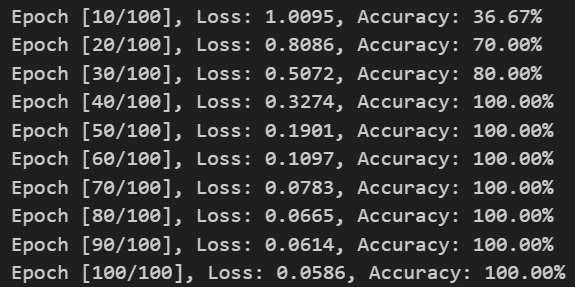
\includegraphics[width=0.7\textwidth]{./assets/MLP-training.png}
    \caption{Training loss and accuracy of the MLP over 100 epochs.}
    \label{fig:mlp-training}
\end{figure}

Accuracy on the test set reached 100\% after 100 epochs of training.
\begin{figure}[H]
    \centering
    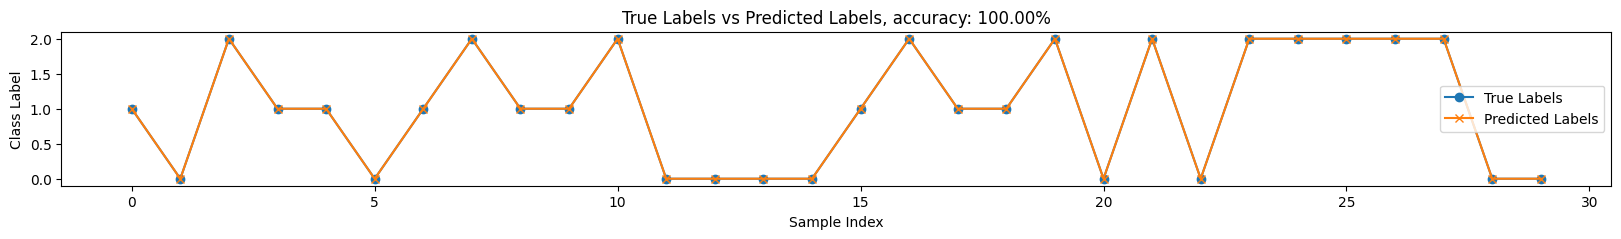
\includegraphics[width=0.9\textwidth]{./assets/MLP-accuracy.png}
    \caption{Accuracy of the MLP on the test set after 100 epochs of training.}
    \label{fig:mlp-accuracy}
\end{figure}

\subsection{Exporting Parameters}
The trained model's parameters were exported to be hardcoded into the \texttt{C} implementation. The weights and biases of each layer were extracted and saved in a format compatible with the hardware implementation.
\begin{lstlisting}[language=Python]
# Export the trained model's parameters
weights = {name: param.detach().numpy() for name, param in model.named_parameters()}

with open('weights.txt', 'w') as f:
    for name, weight in weights.items():
        f.write(f"{name}\n")
        np.savetxt(f, weight, fmt='%f')
\end{lstlisting}

\subsection{Implementation}
The forward pass for an MLP is implemented in \texttt{C} using a sequence of functions for each layer type. The function takes four input features and processes them through three layers, each with its own weights and biases. The output is the predicted class index.

The forward pass function is defined as follows:
\begin{lstlisting}
int forward(float input0, float input1, float input2, float input3) {
    const int input_sizes[4] = {4, 10, 10, 3};
    const int num_layers = 3;

    float current_input[MAX_NEURONS];
    float next_input[MAX_NEURONS];

    current_input[0] = input0;
    current_input[1] = input1;
    current_input[2] = input2;
    current_input[3] = input3;

    for (int i = 0; i < num_layers; i++) {
        #pragma HLS UNROLL
        Layer *layer = &mlp.layers[i];
        for (int j = 0; j < input_sizes[i + 1]; j++) {
            float sum = layer->biases[j];
            
            for (int k = 0; k < input_sizes[i]; k++) {
                sum += layer->weights[j][k] * current_input[k];
            }
            next_input[j] = reLu(sum);
        }

        for (int j = 0; j < input_sizes[i + 1]; j++) {
            current_input[j] = next_input[j];
        }
    }

    int max_index = 0;
    float max = current_input[0];
    for (int i = 1; i < NUM_CLASSES; i++) {
        #pragma HLS UNROLL
        if (current_input[i] > max) {
            max = current_input[i];
            max_index = i;
        }
    }
    return max_index;
}
\end{lstlisting}


\section{Results}
TODO

\section{Conclusions}
TODO

\end{document}


